% !TEX TS-program = pdflatex
% !TEX encoding = UTF-8 Unicode

% This is a simple template for a LaTeX document using the "article" class.
% See "book", "report", "letter" for other types of document.

\documentclass[11pt]{article} % use larger type; default would be 10pt
\usepackage{ifthen}
\usepackage[utf8]{inputenc} % set input encoding (not needed with XeLaTeX)
% packages
\usepackage{xspace}
\usepackage{ifthen}
\usepackage{amsbsy}
\usepackage{amssymb}
\usepackage{balance}
\usepackage{booktabs}
\usepackage{graphicx}
\usepackage{multirow}
\usepackage{needspace}
\usepackage{microtype}
\usepackage{bold-extra}
\usepackage{subfigure}
\usepackage{wrapfig}

%%% Examples of Article customizations
% These packages are optional, depending whether you want the features they provide.
% See the LaTeX Companion or other references for full information.

%%% PAGE DIMENSIONS
\usepackage{geometry} % to change the page dimensions
\geometry{a4paper} % or letterpaper (US) or a5paper or....
% \geometry{margins=2in} % for example, change the margins to 2 inches all round
% \geometry{landscape} % set up the page for landscape
%   read geometry.pdf for detailed page layout information

\usepackage{graphicx} % support the \includegraphics command and options

% \usepackage[parfill]{parskip} % Activate to begin paragraphs with an empty line rather than an indent

%%% PACKAGES
\usepackage{booktabs} % for much better looking tables
\usepackage{array} % for better arrays (eg matrices) in maths
\usepackage{paralist} % very flexible & customisable lists (eg. enumerate/itemize, etc.)
\usepackage{verbatim} % adds environment for commenting out blocks of text & for better verbatim
\usepackage{subfig} % make it possible to include more than one captioned figure/table in a single float
% These packages are all incorporated in the memoir class to one degree or another...

%%% HEADERS & FOOTERS
\usepackage{fancyhdr} % This should be set AFTER setting up the page geometry
\pagestyle{fancy} % options: empty , plain , fancy
\renewcommand{\headrulewidth}{0pt} % customise the layout...
\lhead{}\chead{}\rhead{}
\lfoot{}\cfoot{\thepage}\rfoot{}

% proof-reading
\usepackage{xcolor}
\usepackage[normalem]{ulem}
\newcommand{\ra}{$\rightarrow$}
\newcommand{\ugh}[1]{\textcolor{red}{\uwave{#1}}} % please rephrase
\newcommand{\ins}[1]{\textcolor{blue}{\uline{#1}}} % please insert
\newcommand{\del}[1]{\textcolor{red}{\sout{#1}}} % please delete
\newcommand{\chg}[2]{\textcolor{red}{\sout{#1}}{\ra}\textcolor{blue}{\uline{#2}}} % please change
\newcommand{\chk}[1]{\textcolor{ForestGreen}{#1}} % changed, please check

% comments \nb{label}{color}{text}
\newboolean{showcomments}
\setboolean{showcomments}{true}
\ifthenelse{\boolean{showcomments}}
	{\newcommand{\nb}[3]{
		{\colorbox{#2}{\bfseries\sffamily\scriptsize\textcolor{white}{#1}}}
		{\textcolor{#2}{\sf\small$\blacktriangleright$\textit{#3}$\blacktriangleleft$}}}
	 \newcommand{\version}{\emph{\scriptsize$-$Id$-$}}}
	{\newcommand{\nb}[2]{}
	 \newcommand{\version}{}}
\newcommand{\rev}[2]{\nb{Reviewer #1}{red}{#2}}
\newcommand{\ab}[1]{\nb{Alexandre}{blue}{#1}}
\newcommand{\sv}[1]{\nb{Santiago}{orange}{#1}}

%%% SECTION TITLE APPEARANCE
\usepackage{sectsty}
\allsectionsfont{\sffamily\mdseries\upshape} % (See the fntguide.pdf for font help)
% (This matches ConTeXt defaults)

%%% ToC (table of contents) APPEARANCE
\usepackage[nottoc,notlof,notlot]{tocbibind} % Put the bibliography in the ToC
\usepackage[titles,subfigure]{tocloft} % Alter the style of the Table of Contents
\renewcommand{\cftsecfont}{\rmfamily\mdseries\upshape}
\renewcommand{\cftsecpagefont}{\rmfamily\mdseries\upshape} % No bold!

%%% END Article customizations

%%% The "real" document content comes below...

\title{Patterns Summary}

\date{} % Activate to display a given date or no date (if empty),
         % otherwise the current date is printed 

\begin{document}
\maketitle

\section{Uni-Class Patterns}

\subsection{Implemented}
\begin{itemize}
\item Idle Class: This uni-class pattern looks for all the classes that have not been changed for an X number of versions. Specifically, the uni-class pattern returns all the class versions in which this behavior occurs. For example, if a system has 10 versions and the class A was modified in versions 1, 4, and 10 the uni-class pattern will be true in the following versions whit X=3: 4, 7, 8, and 9.  
\item Most Complex Classes: This uni-class pattern looks for all the versions of the classes in which a class was in the X\% of the most complex classes of a system. To calculate the complexity of a class the metric Weighted Method Count (WMC) is used.   
\item Supernova: This uni-class pattern is related with the categorization proposed by Lanza. This milestone identifies those versions of a class in which it grows more than X\% regarding it previous version. 
\end{itemize}

\subsection{Not Implemented}
\begin{itemize}
\item Ghost Methods: A method that was deleted in a version is added again in a posterior version.
\item Duplicated Code: An index that measure the code duplication in a system increases a X\%  regarding it previous version.
\item Complex method: A method that is in the X\% of the most complex methods of a system was added.
\item Fan-In Indicator: A method has a fan-in higher than X.
\item Dead Method: A method with fan-in=0. \ab{I am not sure that a method with fan-in = 0 is a dead method. Imagine a method that simply return a value?} \sv{Hmmm, yep, you're right}
\item \ab{fanoutCalls = average number of calls a method makes. Measure the amount of external calls a class/method does. }. \sv{Why the average instead of the number of call?}
\item Empty Method: This uni-class pattern looks for all the methods that are defined empty. This may be because they were defined to be implemented in the future\ab{In ArgoUML there are large classes with only empty methods} \sv{Do you know why?}
\end{itemize}

\section{Multi-Class Patterns}
\ab{I do not really understand this section and the figure. Pick a simple example. For example, the evolution of the amount of used classes per class. } \sv{Pero eso no explicaria como funciona el algoritmo de Multi-class. La idea es que un multi-class parttern esta formardo por 2 o mas uni-class patterns que se encuentran en un componente}
\ab{Things that could be interesting to verify, is there a correlation between an increase of the cyclomatic complexity and the amount of dependent classes? My gut feeling says that a class that has an increase of the complexity cyclomatic has also an increase of the amount of dependent classes.} \sv{What do you mean by 'dependent classes'?}

\subsection{The pattern algorithm}
A multi-class pattern is composed by at least two uni-class patterns that occur in the same component. This occurrences can exist in the same or different versions. In order to determine the total number of versions considered to define a multi-class pattern, the pattern algorithm uses a threshold value where \emph{threshold>=0}. 
Consider the model history of the components shown in Figure \ref{fig:exampleOfPatterns}. In this case the history of 6 components is shown where each of them has 7 versions. Also, in this case are used four uni-class patterns.  
\begin{figure}
  \centering
    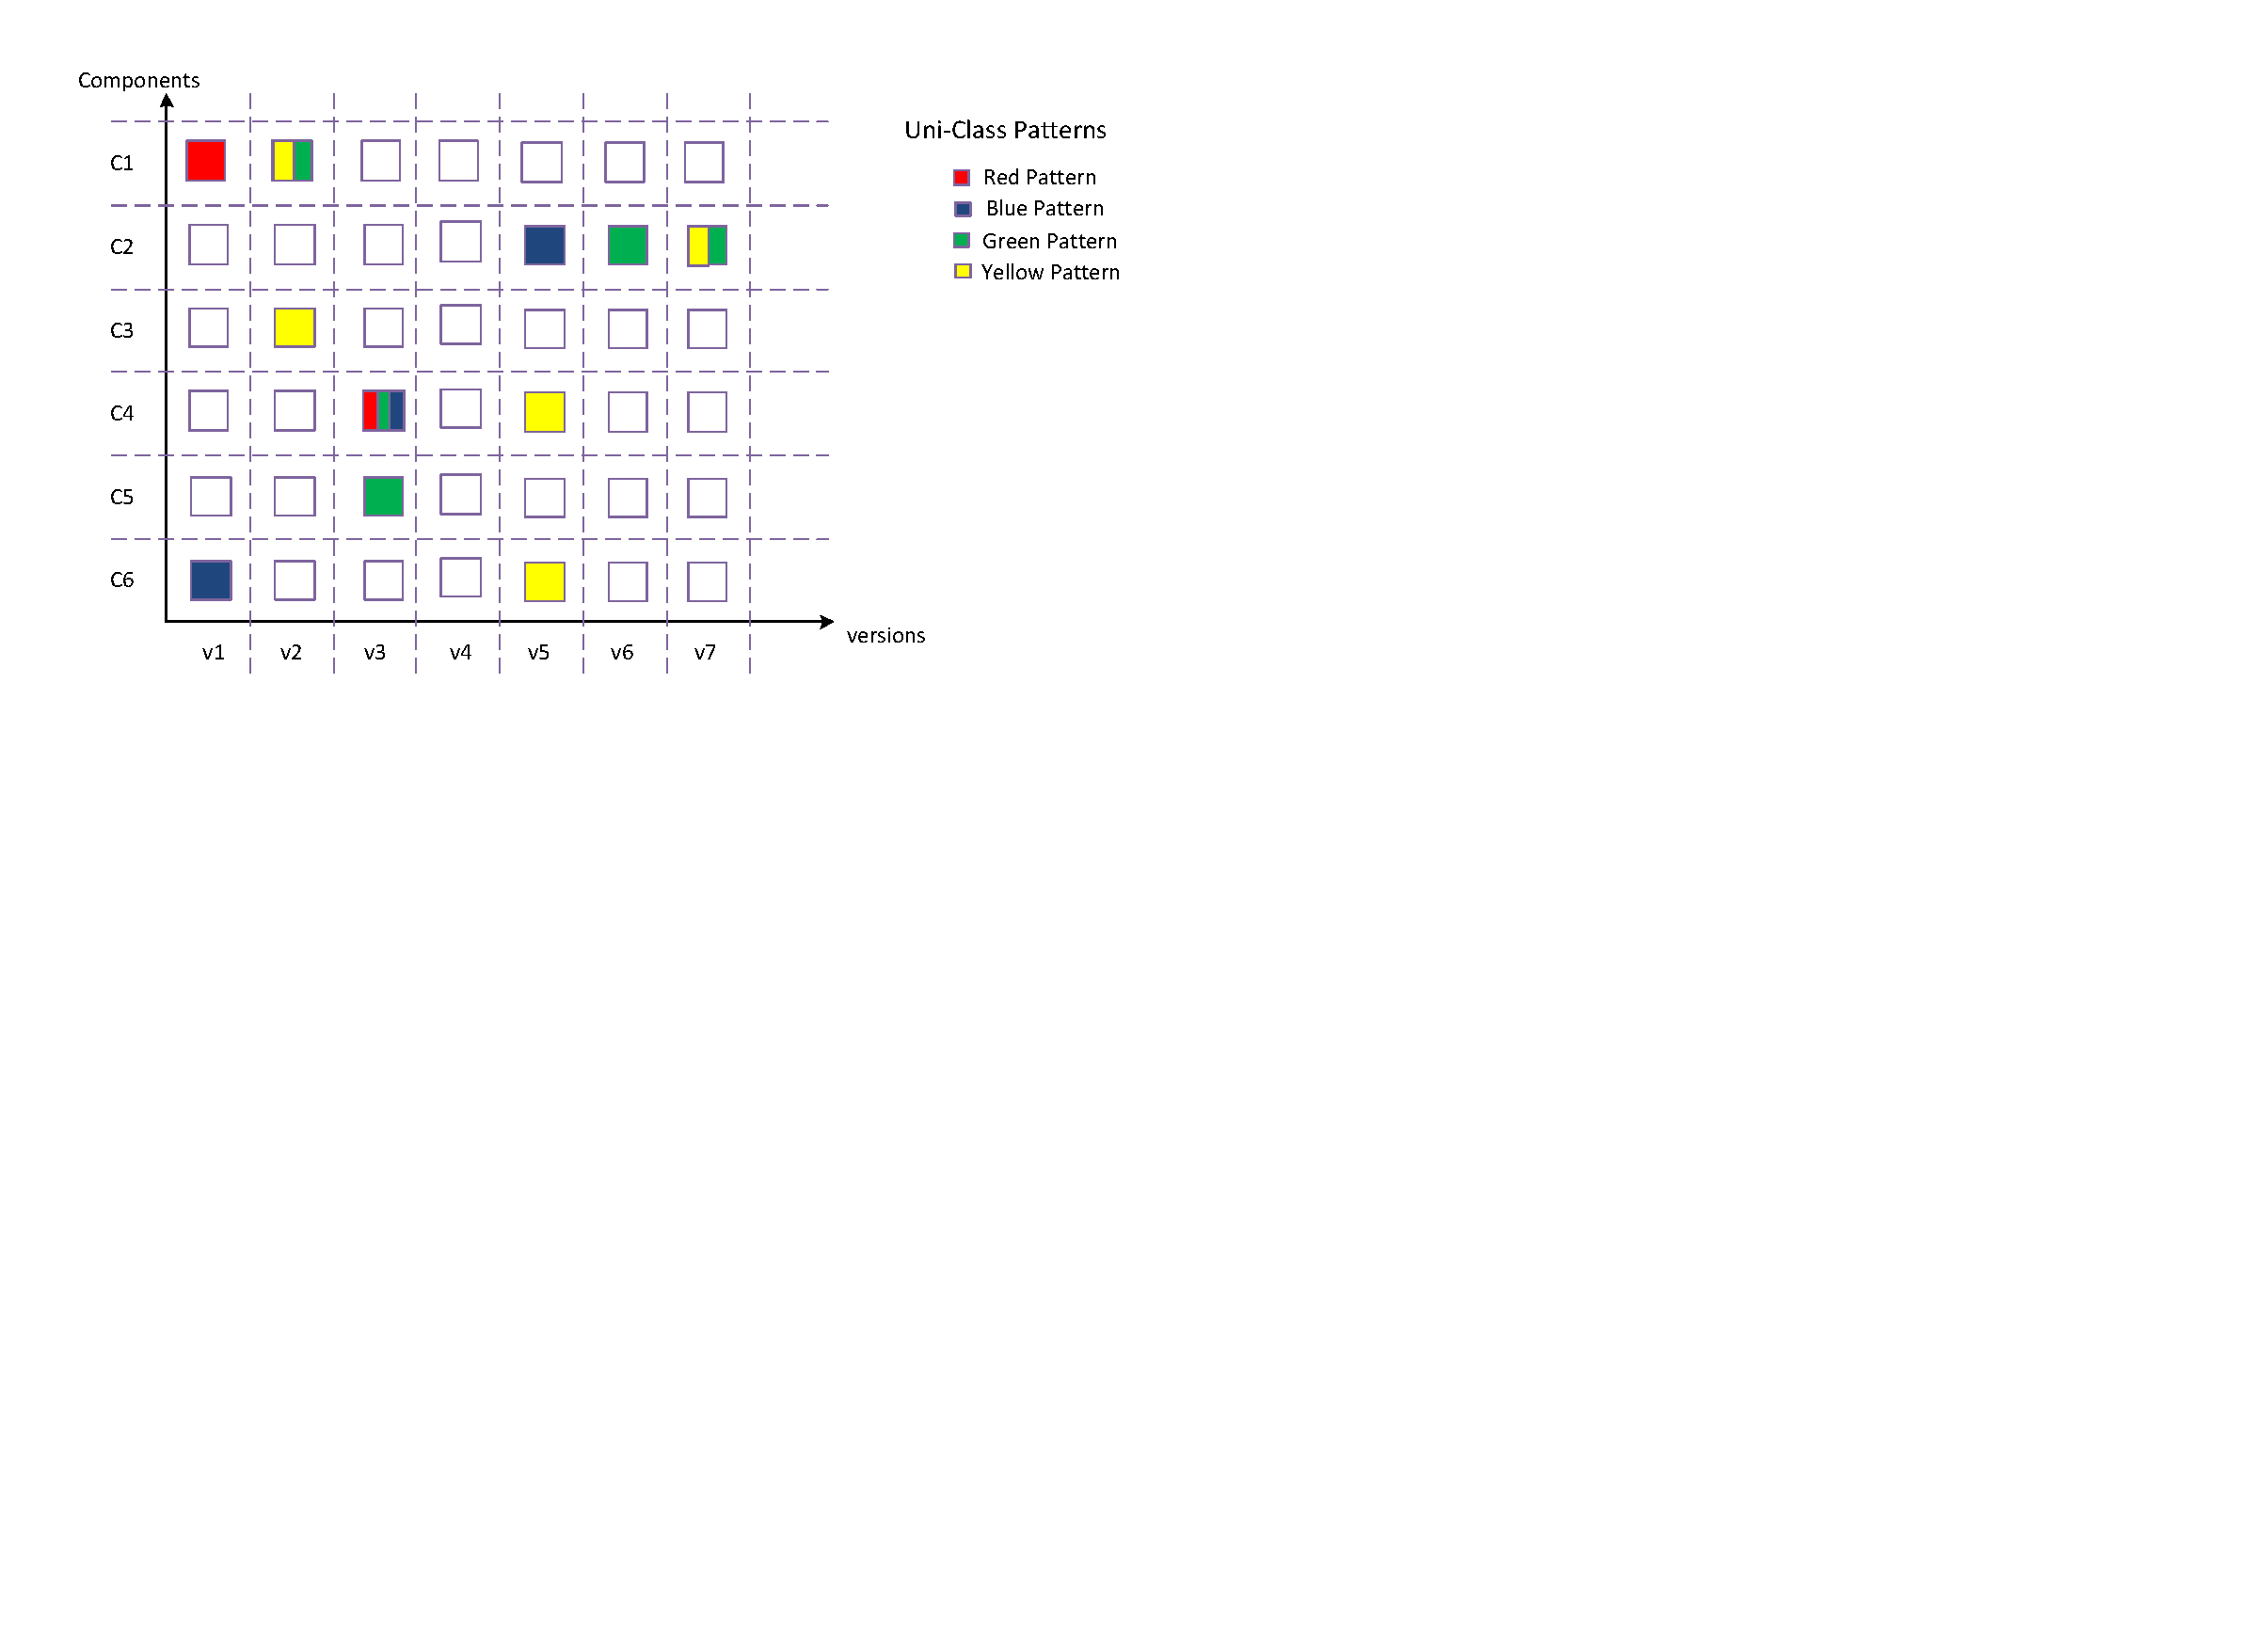
\includegraphics[bb=25bp 490bp 580bp 810bp,clip,scale=0.75]{patterns}
  \caption{Pattern Example}
  \label{fig:exampleOfPatterns}
\end{figure}

When the algorithm is run using the proposed model history, it will return as its output a set of multi-class pattern. For example if the algorithm is run with threshold=0, then all the pattern will be composed by uni-class patterns that occur in a same version. In this case the patterns obtained will be: 
\begin{itemize}
\item \{[Yellow, v2], [Green, v2], C1\}
\item \{[Yellow, v7], [Green, v7], C2 \}
\item \{[Red, v3], [Green, v3], [Blue, v3], C4\}
\end{itemize}

If the algorithm is executed with  threshold=1, the output will be the patterns found when the algorithm was run with threshold=0 plus:
\begin{itemize}
\item \{[Red, v1], [Yellow, v2], [Green, v2], C1\}
\item \{[Blue, v5], [Green, v6], [Yellow, v7], [Green, v7], C2\}
\end{itemize}

Finally, if threshold=2, the returned patterns will be the same of threshold=0 and threshold=1 plus:
\begin{itemize}
\item \{[Red, v3], [Green, v3], [Blue, v3], [Yellow, v5], C4\}
\end{itemize}

\subsection{Identified Patterns}
\end{document}
